\section{Modeling}\label{sec:modeling}
One of the most pressing questions related to this work is whether or not the
increased star-to-star variability in the activity metric and the Jao Gap,
which are coincident in magnitude, are driven by the same underlying mechanism.
The challenge when addressing this question arrises from current computational
limitations. Specifically, the kinds of three dimensional
magneto-hydrodynamical simulations --- which would be needed to derive the
effects of convective kissing instabilities on the magnetic field of the star
--- are infeasible to run over gigayear timescales while maintaing thermal
timescale resolutions needed to resolve periodic mixing events.

In order to address this and answer the specific question of \textit{could
kissing instabilities result in increased star-to-star variability of the
magnetic field}, we adopt a very simple toy model. Kissing instabilities result
in transient radiative zone seperating the core of a star (convective) from its
envelope (convective). When this radiative zone breaks down two important
things happen: one, the entire star becomes mechanically coupled, and two, convective
currents can now move over the entire radius of the star. \citet{Jao2023}
propose that this mecahnical coupling may allow the stars core to act as an
angular momentum sink thus accelerating a stars spin down and resulting in
anomolously low H$\alpha$ emission. 

Regardless of the exact mechanism by which the magnetic field may be effected,
it it reasonable to expect that both the mechanical coupling and the change to
the scale of convective currents will have some effect on the stars magnetic
field. On a microscopic scale both of these will change how packets of charge
within a star move and may serve to disrupt a stable dynamo. Therefore, in the
model we present here we make only one primary assumption: \textit{every mixing
event may modify the stars magnetic field by some amount}. Within our model
this assumption manifests as a random linear perturbation applied to some base
magnetic field at every mixing event. The strength of this perturbation is 
sampled from a normal distrubution with some standard deviation, $\sigma_{B}$.

Synthetic stars are sampled from a grid of stellar models evolved using the
Dartmouth Stellar Evolution Program (DSEP). Each stellar model was evolved
using a high temporal resolution (timesteps no larger than 10,000 years
{\color{red} Check this}) and typical numerical tolernances of one part in
$10^5$. Each model was based on a GS98 ({\color{red} CITATION}) solar
composition with a mass range from 0.3 M$_{\odot}$ to 0.4 M$_{\odot}$. Finally,
models adopt OPLIB high temperature radiative opacities, Ferguson 2004 low
temperature radiative opacities, and include both atomic diffusion and
gravitational settling. A Kippenhan-Iben diagram showing the structural
evolution of a model within the gap is shown in Figure \ref{fig:kippenhan}.

\begin{figure*}
  \centering
  \includegraphics[width=0.9\textwidth]{figures/Kippenhan_clamped.pdf}
  \caption{Kippenhan-Iben diagram for a 0.345 solar mass star. Note the
  periodic mixing events (where the plotted curves peak).}
  \label{fig:kippenhan}
\end{figure*}

Each synthetic star is assigned some base magnetic activiy ($B_{0} \sim
\mathcal{N}(1, \sigma_{B})$) and then the number of mixing events before some age $t$
are counted based on local maxima in the core temperature. The toy magnetic
activiy at age $t$ for the model is given in Equation \ref{eqn:activity}. An
example of the magnetic evolution resulting from this model is given in Figure
\ref{fig:simpleB}. Fundamentally, this model presents magnetic
activity variation due to mixing events as a random walk and therefore results will
increasingly divergence over time.

\begin{align}\label{eqn:activity}
  B(t) = B_{0} + \sum_{i}B_{i} \sim \mathcal{N}(1, \sigma_{B}) 
\end{align}

\begin{figure}
  \centering
  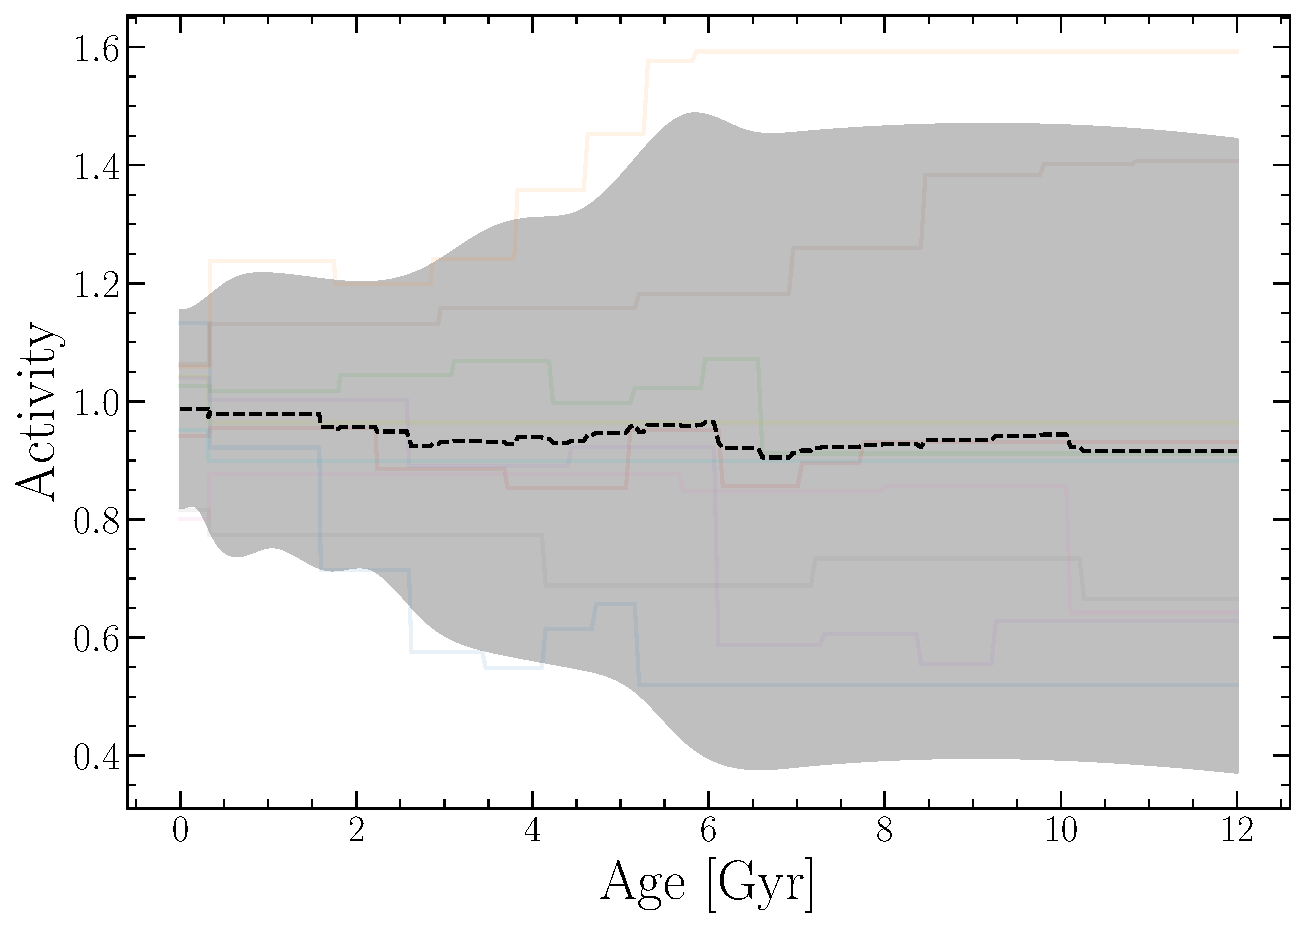
\includegraphics[width=0.45\textwidth]{figures/simpleBEvolution.pdf}
  \caption{Example of the toy model presented here resulting in increased
  divergence between stars magnetic fields. The shaded region represents the
  maxium spread in the two point correlation function at each age.}
  \label{fig:simpleB}
\end{figure}

Applying the same analysis to these models as was done to the observations as
described in Section {\color{red} X.X} we find that this simple model results
in a qualitatively similar trend in the standard deviation vs. magnitude graph.
The interpretation here is important, what this qualitative similarity
demonstrates is that it may be reasonable to expect kissing instabilities to
result in the observed increased star-to-star variation. Importantly, we are
not able to claim that kissing instabilities \textit{do} lead to these
increased variations, only that they reasonably could. Further modeling,
observational, and theoretical efforts will be needed to more definitivley
answer this question.
